\documentclass{article}

\usepackage{ctex}
\usepackage{tikz}
\usetikzlibrary{automata, positioning, arrows}
\usetikzlibrary{cd}

\usepackage{amsthm}
\usepackage{amsmath}
\usepackage{amssymb}
%\usepackage{stmaryrd}
\usepackage{mathtools}
\usepackage{proof}

\usepackage[linesnumbered,ruled,vlined]{algorithm2e}

\usepackage[cache=false]{minted} %code block

%\usepackage{unicode-math}
\PassOptionsToPackage{hyphens}{url}\usepackage{hyperref} %url解决过长的问题
\usepackage{hyperref} %url
\hypersetup{
    colorlinks=true,
    linkcolor=blue,
    filecolor=magenta,      
    urlcolor=cyan,
    pdftitle={Overleaf Example},
    pdfpagemode=FullScreen,
    }


\usepackage[textwidth=18cm]{geometry} % 设置页宽=18

\usepackage{blindtext}
\usepackage{bm}
\parindent=0pt
\setlength{\parindent}{2em} 
\usepackage{indentfirst}

\usepackage{xcolor}
\usepackage{titlesec}
\titleformat{\section}[block]{\color{blue}\Large\bfseries\filcenter}{}{1em}{}
\titleformat{\subsection}[hang]{\color{red}\Large\bfseries}{}{0em}{}
%\setcounter{secnumdepth}{1} %section 序号

\newtheorem{theorem}{Theorem}[section]
\newtheorem{lemma}[theorem]{Lemma}
\newtheorem{corollary}[theorem]{Corollary}
\newtheorem{proposition}[theorem]{Proposition}
\newtheorem{example}[theorem]{Example}
\newtheorem{definition}[theorem]{Definition}
\newtheorem{remark}[theorem]{Remark}
\newtheorem{exercise}{Exercise}[section]
\newtheorem{annotation}[theorem]{Annotation}


%{\mathlarger{\mathlarger\mathlarger{\mathlarger{\oldPi}}}}

\newcommand\Set[2]{\{\,#1\mid#2\,\}} %集合
\newcommand\SET[2]{\Set{#1}{\text{#2}}} %

\newcommand{\redt}[1]{\textcolor{red}{#1}}
\newcommand{\bluet}[1]{\textcolor{blue}{#1}}
\newcommand{\abracket}[1]{\ensuremath{\left< #1 \right>}}

\newcommand*{\xfunc}[4]{{#2}\colon{#3}{#1}{#4}}
\newcommand*{\func}[3]{\xfunc{\to}{#1}{#2}{#3}}


\newcommand{\inl}[1]{\ensuremath{\text{inl}~#1}}
\newcommand{\inr}[1]{\ensuremath{\text{inr}~#1}}
\newcommand{\fold}[1]{\ensuremath{{fold}_{#1}}}
\newcommand{\unfold}[1]{\ensuremath{{unfold}_{#1}}}
\newcommand{\lam}[2]{\ensuremath{\lambda #1\ldotp #2}} %lamx.y
\newcommand{\pair}[1]{\ensuremath{\left\langle#1\right\rangle}}
\newcommand{\projone}[1]{\ensuremath{#1.1}}
\newcommand{\projtwo}[1]{\ensuremath{#1.2}}
\newcommand{\caseof}[3]{\ensuremath{{\textbf{case}}~#1~{\textbf{of}}~\inl{x_1}\mapsto #2\mid\inr{x_2}\mapsto #3}}
\newcommand{\Lam}[2]{\ensuremath{\Lambda #1\ldotp #2}}
\newcommand{\pack}[3]{\ensuremath{{pack}~\pair{#1,#2}~{as}~#3}}
\newcommand{\unpack}[4]{\ensuremath{{unpack}~#1~{as}~\pair{#2,#3}~{in}~#4}}
\newcommand{\assign}[2]{\ensuremath{#1~\coloneqq~#2}}
\newcommand{\singletype}[1]{\text{#1}}
\newcommand{\termtype}[2]{\ensuremath{#1:#2}}
\newcommand{\type}[3]{\ensuremath{ \left\{#1:#2\relmiddle|#3 \right\}}}
\newcommand{\matgen}[2]{\ensuremath{\mu #1\ldotp#2}} %ux.y
\newcommand{\mat}[0]{\matgen{\alpha}{\tau}} %ua.t
\newcommand{\fatgen}[2]{\ensuremath{\forall #1\ldotp#2}}
\newcommand{\fat}[0]{\fatgen{\alpha}{\tau}}
\newcommand{\eatgen}[2]{\ensuremath{\exists #1\ldotp#2}}
\newcommand{\eat}[0]{\eatgen{\alpha}{\tau}}
\newcommand{\fatgent}[2]{\ensuremath{\trgb{\forall} #1\ldotp#2}}
\newcommand{\fatt}[0]{\fatgent{\alpt}{\tat}}
\newcommand{\eatgent}[2]{\ensuremath{\trgb{\exists} #1\ldotp#2}}
\newcommand{\eatt}[0]{\eatgent{\alpt}{\tat}}

\newcommand{\fail}[0]{\mi{fail}}

\newcommand{\bnfdef}[0]{\ensuremath{\mathrel{::=}}} %::=
\newcommand{\term}[1]{\ensuremath\mathsf{#1}}
\newcommand{\true}{\term{true}}
\newcommand{\false}{\term{false}}
\newcommand{\ifelse}[3]{\ensuremath{\textbf{if}~#1~\textbf{then}~#2~\textbf{else}~#3}}
\newcommand{\newwhiledo}[2]{\ensuremath{\textbf{while}~#1~\textbf{do}~#2}}
\newcommand{\letvar}[2]{\ensuremath{\textbf{letvar}~#1~\textbf{in}~#2}}
\newcommand{\succt}[1]{\term{succ}~#1}
\newcommand{\pred}[1]{\term{pred}~#1}
\newcommand{\iszero}[1]{\term{iszero}~#1}
\newcommand{\seq}[2]{#1;#2}
\newcommand{\subtyp}[2]{#1<:#2}

\newcommand{\dbracket}[1]{\ensuremath{\left\llbracket\,\vcenter{\hbox{$#1$}}\,\right\rrbracket}}

\newcommand{\todo}[1]{\textcolor{red}{TODO: #1}\PackageWarning{TODO:}{#1!}}

\newcommand{\defeqv}{\vcentcolon\equiv}

%variable name
\ExplSyntaxOn 
\NewDocumentCommand{\vn}{m}
 {
   \seq_set_split:Nnn \l_tmpa_seq { ~ } { #1 }
   \int_compare:nTF { \seq_count:N \l_tmpa_seq > 1 }
    {
     \seq_set_map:NNn \l_tmpb_seq \l_tmpa_seq { \exp_not:N \mathit { ##1 } }
     (\seq_use:Nn \l_tmpb_seq { \  })
    }
    { \mathop{}\!\mathit{#1} }
 }
\ExplSyntaxOff


\begin{document}
\title{关于Maple Algebra的这一路}
\author{枫聆 (maplegra)}
\maketitle
\tableofcontents
\newpage

\section{Logic}

\subsection{Classic Logic}

\begin{annotation}
\rm Double negation和excluded middle是logical equivalent, 关于它们有两个通俗解释:
\begin{itemize}
	\item Double negation: 如果你想证明$P$为$true$, 只需要说明$P$不是$false$即可.
	\item Excluded middle: 任意一个命题$P$, 它不是$true$就是$false$.
\end{itemize}
\end{annotation}

\subsection{Higher-order logic}

\begin{annotation}
\rm Second-order logic在first-order logic的基础上,给其中的谓词也加上了量词. 给谓词加量词意义是什么呢? 谓词实际上可以理解为varibles的properties,所以相当于你给variable's properties也加上了量词. 形如:
\[
	\exists P.\ P(b)
\]
这里的$P$可以看做一个谓词变量(predicate variable). 从语义上来说$P$可以理解为集合,更进一步说就是满足某种property的varibles组成的set, 所以你对$P$施加一个量词也就是在考虑不同的集合,此时上面的formula可以非正式地理解为存在某个集合$P$包含$b$.
\end{annotation}

\subsection{Misc}

\begin{definition}
\rm A set of logical connectives is called \redt{functionally complete} if every boolean expression is equivalent to one involving only these connectives.
\end{definition}

\begin{definition}
\rm 简而言之,如果任意的logical formula都可以只用给定的一些logical connectives来构造一个等价的新的logical formula, 我们就说这些这些logical connectives组成的system是functionally complete. 
\end{definition}

\begin{example}
\rm 列举一些在classic logic下functionally complete的system:
\begin{itemize}
	\item $\{\downarrow\}$, $\{\uparrow\}$, 其中$\downarrow$表示$A \downarrow B = \neg (A \vee B)$, $\uparrow$表示$A \uparrow B = \neg (A \wedge B)$.
	\item $\{\vee ,\neg \}$, $\{\wedge ,\neg \}$, etc.
	\item $\{\land ,\lor ,\rightarrow \}$, etc.
\end{itemize}
\end{example}

\section{Language}

\subsection{Standard Semantics}

\begin{annotation}
\rm Operational semantics关注给定一个initial state会得到怎样的final state, 每一个CFG's node对应一个transfer function $f:\mathcal{S} \to \mathcal{S}$
\[
	\lam{s}{(\mu(s),next)}.
\]
其中$f$表示对state $s$的update, next表示下一个将要进入的node. 那么operational semantics的一个解释过程可以用递归的形式定义:
\[
	\vn{interp} = \lam{s}{\lam{n}{\ifelse{isExitNode(n)}{s}{\mathbf{let}~(s',n')=f_n(s)~\mathbf{in}~\vn{interp}~s'~n'}}}
\]
如果我们希望得到一个准确的定义,即不希望等式两边都包含$\vn{interp}$,那么我可以利用一个trick
\[
\vn{semantics} = \vn{fix}(\lam{F}{\lam{s}{\lam{n}{\ifelse{isExitNode(n)}{s}{\mathbf{let}~(s',n')=f_n(s)~\mathbf{in}~F~s'~n'}}}})
\]
你仔细观察一下这个fixpoint就是$\vn{interp}$本身.
\end{annotation}

\subsection{Collecting Semantics}

\begin{annotation}
\rm Collecting semantics和operational semantics不同的是,每一个CFG's node可能对应了一个set of states, 而不是单一的state了. 因为collecting semantics从一开始就把所有可能的initial states作为了一个set来考虑. 因此此时的transfer function为$f:\mathcal{P}(\mathcal{S}) \to \mathcal{P}(\mathcal{S})$:
\[
f_{n \to m} = \lam{S}{\Set{s'}{s \in S ~\text{and}~f_n(s)=(s',m)}}
\]
\end{annotation}

\subsection{Language equation and Arden's Rule}

\begin{theorem}
\rm The set $A^* \cdot B$ is the smallest language that is a solution for $X$ in the linear equation 
\[
	X = A \cdot X + B
\]
where $X, A, B$ are sets of string and $+$ stands for union of languages. Moreover, If the set $A$ does not contain the empty word, then the solution is unique.
\end{theorem}

\begin{annotation}
\rm \bluet{Arden's rule can be used to help convert some finite automatons to regular expressions}.
\end{annotation}



\newpage
\section{Equivalence of Program}

\subsection{Graph Ismorphism}

\subsection{Accepted Language Equivalentce}

\begin{annotation}
\rm \cite{CCS} Chapter 1.
\end{annotation}

\subsection{Bisimulation and Observation Equivalence}

\begin{definition}
\rm A labelled transition system (LTS) is a tuple $(S, \Lambda, \to)$ where $S$ is set of states, $\Lambda$ is set of labels, and $\to$ is relation of labelled transitions (i.e., a subset of $S \times \Lambda \times S$).  A $(p,\alpha,q) \in \to$ is written as $p  \xrightarrow{\alpha} q$. 
\end{definition}

\begin{annotation}
\rm \todo{categorical semantics: $F$-coalgebra}
\end{annotation}


\begin{definition}
\rm \cite{ITLTS}Let $T=(S,\Lambda,\to)$ be a labelled transition system. The set of \redt{traces} $\vn{Tr}(s)$, for $s \in S$ is the minimal set satisfying
\begin{itemize}
	\item $\varepsilon \in \vn{Tr}(s)$.
	\item $\alpha~\sigma \in \vn{Tr}(s)$ if $\Set{s' \in S}{s~ \xrightarrow{\alpha}~s' ~\text{and}~\sigma \in \vn{Tr}(s')}$. 
\end{itemize}
\end{definition}

\begin{definition}
\rm Two states $p,q$ are trace equivalent iff $\vn{Tr}(p) = \vn{Tr}(q)$.
\end{definition}

\begin{definition}
\rm (\redt{Simultation}) Given two labelled transition system $(S_1, \Lambda, \to_1)$ and $(S_2, \Lambda, \to_2)$, relation $R \subseteq S_1 \times S_2$ is a simulation iff, for all $(p,q) \in R$ and $\alpha \in \lambda$ satisfies
\[
	\text{for any}~p \xrightarrow{\alpha}_1 p', ~\text{then there exists}~ q'~\text{such that}~q \xrightarrow{\alpha}_2 q'~\text{and}~(p',q') \in R 	
\]
\begin{center}
% https://tikzcd.yichuanshen.de/#N4Igdg9gJgpgziAXAbVABwnAlgFyxMJZABgBpiBdUkANwEMAbAVxiRDRAF9T1Nd9CKACzkqtRizZoA5Fx7s+eAkTIBmMfWatEIAI5ze2JYOQj11TZJ27ZnMTCgBzeEVAAzAE4QAtkjIgcCCQARgsJbRAAHUjGNAALOgMQTx8kACZqQKRVMK02aNiEkGoGOgAjGAYABUUBNg8sRzicYpAGLDAIuAh2qCSU30R-LMQMto6IqDo4OIdW2bo+xDAmBgZcqxAAJVbSiura5R0GppbMuiwGNkhO-q9B0ICgxBzx250pmbnqBaWVtY2ER2dk4QA
\begin{tikzcd}
p \arrow[rrrr, "\alpha"] \arrow[ddd, "R"', dashed] &  &  &  & p' \arrow[ddd, "R", dashed] \\
                                                   &  &  &  &                             \\
                                                   &  &  &  &                             \\
q \arrow[rrrr, "\alpha"']                          &  &  &  & q'                         
\end{tikzcd}
\end{center}
\end{definition}

\begin{definition}
\rm We say $q$ simulates $p$ if there exists a simulation $R$ includes $(p,q)$ (i.e., $(p,q) \in R$), written $p < q$.
\end{definition}

%\begin{lemma}
%\rm The simulation is reflexive and transitive. 
%\end{lemma}


\begin{definition}
\rm (\redt{Bisimultation}) Given two labelled transition system $(S_1, \Lambda, \to_1)$ and $(S_2, \Lambda, \to_2)$, relation $R \subseteq S_1 \times S_2$ is a bisimulation iff both $R$ and its converse $\overline{R}$ are simulations, for all $(p,q) \in R$ and $\alpha \in \Lambda$ satisfies
\[
	\begin{gathered}
	\text{for any}~p \xrightarrow{\alpha}_1 p', ~\text{then there exists}~ q'~\text{such that}~q \xrightarrow{\alpha}_2 q'~\text{and}~(p',q') \in R \\
	\text{for any}~q \xrightarrow{\alpha}_2 q', ~\text{then there exists}~ p'~\text{such that}~p \xrightarrow{\alpha}_1 p'~\text{and}~(p',q') \in R
	\end{gathered} 	
\]
\end{definition}

%\begin{definition}
%\rm A binary relation between state transition systems, associating systems that behave in the same way in that one system simulates the other and vice versa.
%\end{definition}

\begin{example}
\rm 一些bisimulation的例子
\begin{center}
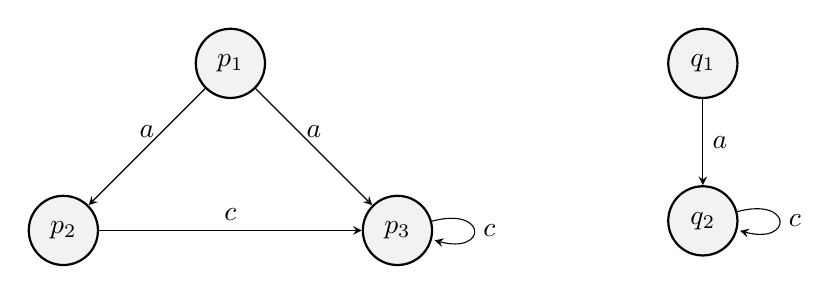
\begin{tikzpicture}
\tikzset{
->, % makes the edges directed
>=stealth, % makes the arrow heads bold
node distance=3cm, % specifies the minimum distance between two nodes. Change if necessary.
every state/.style={thick, fill=gray!10}, % sets the properties for each ’state’ node
initial text=$ $, % sets the text that appears on the start arrow
}
	\node[state] (p1) {$p_1$};
	\node[state, below left of=p1, node distance=3cm] (p2) {$p_2$};
	\node[state, below right of=p1, node distance=3cm] (p3) {$p_3$};
	\node[state, right of=p1, node distance=6cm] (q1) {$q_1$};
	\node[state, below of=q1, node distance=2cm] (q2) {$q_2$};
	
	\draw (p1) edge[above] node{$a$} (p2)
	(p1) edge[above] node{$a$} (p3)
	(p2) edge[above] node{$c$} (p3)
	(p3) edge[loop right] node{$c$} (p3)
	(q1) edge[right] node{$a$} (q2)
	(q2) edge[loop right] node{$c$} (q2);
\end{tikzpicture}
\end{center}
关于上面两个transition system的bisimultaion为$R=\{(p_1,q_1), (p_2,q_2), (p_3,q_2)\}$. 还有一个比较有点特别的例子
\begin{center}
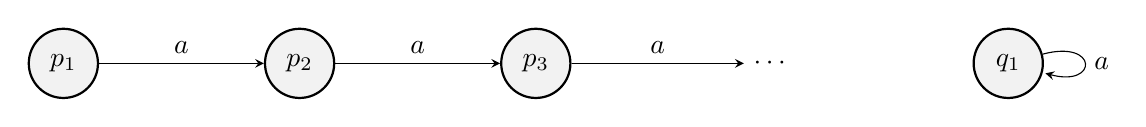
\begin{tikzpicture}
\tikzset{
->, % makes the edges directed
>=stealth, % makes the arrow heads bold
node distance=3cm, % specifies the minimum distance between two nodes. Change if necessary.
every state/.style={thick, fill=gray!10}, % sets the properties for each ’state’ node
initial text=$ $, % sets the text that appears on the start arrow
}
	\node[state] (p1) {$p_1$};
	\node[state, right of=p1, node distance=3cm] (p2) {$p_2$};
	\node[state, right of=p2, node distance=3cm] (p3) {$p_3$};
	\node[right of=p3, node distance=3cm] (p4) {$\cdots$};
	\node[state, right of=p4, node distance=3cm] (q1) {$q_1$};
	
	\draw (p1) edge[above] node{$a$} (p2)
	(p2) edge[above] node{$a$} (p3)
	(p3) edge[above] node{$a$} (p4)
	(q1) edge[loop right] node{$a$} (q1);
\end{tikzpicture}
\end{center}
如果关于上图这样bisimulation $R$存在,那么$(p_i,q_1) \in R$ for every $i$. 再看一个不是bisimulation的例子
\begin{center}
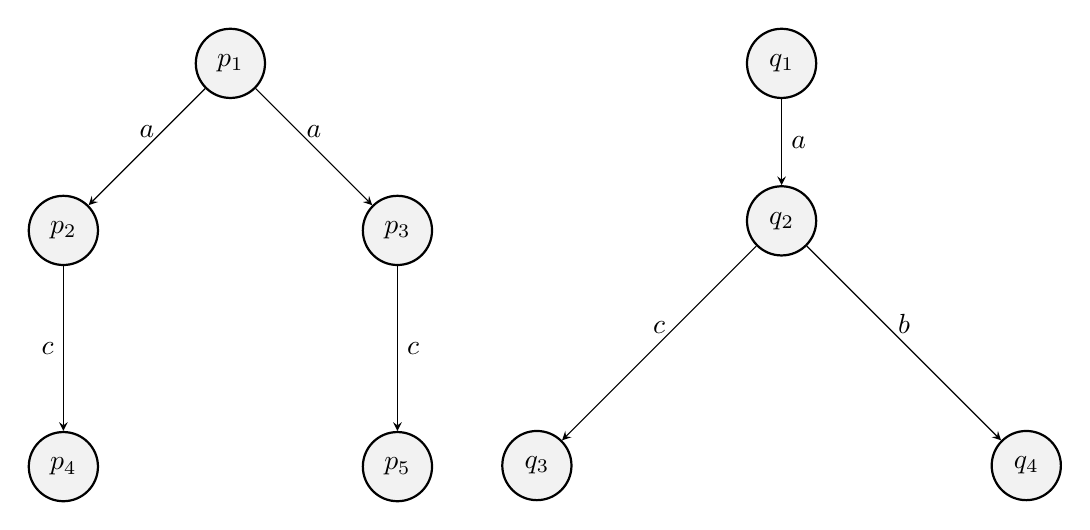
\begin{tikzpicture}
\tikzset{
->, % makes the edges directed
>=stealth, % makes the arrow heads bold
node distance=3cm, % specifies the minimum distance between two nodes. Change if necessary.
every state/.style={thick, fill=gray!10}, % sets the properties for each ’state’ node
initial text=$ $, % sets the text that appears on the start arrow
}
	\node[state] (p1) {$p_1$};
	\node[state, below left of=p1, node distance=3cm] (p2) {$p_2$};
	\node[state, below right of=p1, node distance=3cm] (p3) {$p_3$};
	\node[state, below of=p2, node distance=3cm] (p4) {$p_4$};
	\node[state, below of=p3, node distance=3cm] (p5) {$p_5$};
	\node[state, right of=p1, node distance=7cm] (q1) {$q_1$};
	\node[state, below of=q1, node distance=2cm] (q2) {$q_2$};
	\node[state, below left of=q2, node distance=4.395cm] (q3) {$q_3$};
	\node[state, below right of=q2, node distance=4.395cm] (q4) {$q_4$};
	
	\draw (p1) edge[above] node{$a$} (p2)
	(p1) edge[above] node{$a$} (p3)
	(p2) edge[left] node{$c$} (p4)
	(p3) edge[right] node{$c$} (p5)
	(q1) edge[right] node{$a$} (q2)
	(q2) edge[above] node{$c$} (q3)
	(q2) edge[above] node{$b$} (q4);
\end{tikzpicture}
\end{center}
这里不满足$(p_3, q_2) \notin R$.
\end{example}


\begin{definition}
\rm (\redt{Bisimilarity}) Given two states $p$ and $q$ in $S$, $p$ is bisimilar to $q$, written $p \sim q$,  if and only if there is a bisimulation $R$ such that $(p,q) \in R$. 
\end{definition}

\begin{definition}
\rm The bisimilarity relation $\sim$ is the union of all bisimulations.
\end{definition}

\begin{lemma}
\rm The bisimulation has some properties:
\begin{itemize}
	\item The identity relation $\vn{id}$ is a bisimulation(with two same LTS).
	\item The empty relation $\perp$ is a bisimulation.
	%\item The relation composition $R_1 \circ R_2$ of two bisimulation $R_1$ and $R_2$ is a bisimulation.
	\item (\redt{closed under union}) The $\bigcup_{i \in I} R_i$ of a family of bisimulations $(R_i)_{i \in I}$ is a bisimulation.
\end{itemize}
\end{lemma}

\begin{lemma}
\rm \cite{AITBAC} The bisimilarity relation $\sim$ is equivalence relation (i.e., reflexivity, symmetry, transitivity).
\end{lemma}

\begin{proof}
\rm 其中reflexivity, symmetry是比较显然的. Transitivity稍微麻烦一点,我们用relation composition定义新的relation$R_3 = R_1;R_2$, 此时有$(p,q) \in R_3$,因此只要证明$R_3$ is bisimulation足够了. 取任意一个$(p_1, q_1) \in R_3$,那么按照$R_3$的定义, 存在$(p_1, r_1) \in R_1$和$(r_1, q_1)$. 由$p_1 \sim r_1$那么对于任意的$p_1 \xrightarrow{\alpha} p_1'$, 存在$r_1 \xrightarrow{\alpha} r_1'$满足$(p_1',r_1') \in R_1$. 再由$r_1 \sim q_1$, 存在$q_1 \xrightarrow{\alpha} q_1'$满足$(r_1',q_1') \in R_2$. 于是按照$R_3$的定义也有$(p_1', q_1') \in R_3$. 再由$R_2$ is bisimulation, 从$(r_1,q_1) \in R_2$按照上述的思路往回证明即可,最终$R_3$ is bisimulation.
\end{proof}

\begin{definition}
\rm \cite{mLTS} An LTS is called \redt{deterministic} if for every state $p$ and action $\alpha$, there is at most one state $q$ such that $p \xrightarrow{\alpha} q$.
\end{definition}

\begin{lemma}
\rm In a deterministic LTS, two states are bisimilar if and only if they are trace equivalent,
\[
	s_1 \sim s_2 \iff \vn{Tr}(s_1)=\vn{Tr}(s_2)
\]
\end{lemma}

\begin{proof}
\rm 

先证$\Rightarrow$, 设满足$s_1 \sim s_2$($(s_1,s_2) \in R$ and $R$ is bisimultaion), 设$\sigma_{s_1} \in \vn{Tr}(s_1)$, 其中$\sigma_{s_1}$为sequence $(\alpha_i)_{i \in I}$ where $I$ is a indexed famliy. 由于$s_1 \sim s_2$, 那么对于$s_1 \xrightarrow{\alpha_1} s_1'$, 存在$s_2 \xrightarrow{\alpha_1} s_2'$, 于是$(s_1',s_2') \in R$, 根据$\sigma$长度做induction可以证明$\sigma_{s_1} \in \vn{Tr}(q)$. 再反过来证明$\sigma_{s_2} \in \vn{Tr}(s_2)$也同样有$\sigma_{s_2} \in \vn{Tr}(s_1)$. 最终$\vn{Tr}(s_1)=\vn{Tr}(s_2)$.

对于$\Leftarrow$, 我们可以用$\vn{Tr}(s_1) = \vn{Tr}(s_2)$构造一个bisimulation, 定义relation $R$为
\[
 	\vn{Tr}(s_1) = \vn{Tr}(s_2) \iff (s_1,s_2) \in R.
\]
只要能证明$R$ bisimulation即可. 首先我们来说明在deterministic限制下一个比较好性质: 若$\vn{Tr}(s_1) = \vn{Tr}(s_2)$且当$s_1 \xrightarrow{\alpha} s_1', s_2 \xrightarrow{\alpha} s_2'$, 那么$\vn{Tr}(s_1') = \vn{Tr}(s_2')$. 这样对于任意地$(s_1,s_2) \in R$, 它们accept相同action对应的transition $(s_1', s_2') \in R$. 因此$s_1 \sim s_2$. 
\end{proof}


\begin{definition}
\rm (\redt{Weak Bisimultation}) Given two labelled transition system $(S_1, \Lambda, \to_1)$ and $(S_2, \Lambda, \to_2)$, relation $R \subseteq S_1 \times S_2$ is a bisimulation iff both $R$ and its converse $\overline{R}$ are simulations, for all $(p,q) \in R$ and $\alpha \in \Lambda \cup \{\tau\}$ satisfies
\[
	\begin{gathered}
	\text{for any}~p \xrightarrow{\alpha}_1 p', ~\text{then there exists}~ q'~\text{such that}~q \xrightarrow{\tau*~\alpha~\tau*}_2^* q'~\text{and}~(p',q') \in R \\
	\text{for any}~q \xrightarrow{\alpha}_2 q', ~\text{then there exists}~ p'~\text{such that}~p \xrightarrow{\tau*~\alpha~\tau*}_1^* p'~\text{and}~(p',q') \in R
	\end{gathered} 	
\]
where $\xrightarrow{}^*$ is multi-transition.
\end{definition}


\begin{annotation}
\rm \bluet{对于LTS的一些想法}:
\begin{itemize}
	\item 如果你想用transition system来做reasoning可以考虑把它和Kripke frame联系起来,同时要构造一些modality来设计方便做reasoning的calculus.
	\item (\emph{bisimulation proof method}) 对于两个特别的states来说,我们应该如何找到这样bisimulation来满足$(p,q) \in R$?
	\item 对于两个特别的LTS来说,我们怎样以bisimulation思考它们是否equivalent? bisimulation的最初定义应该叫做strong bisimulation, 它建立的是一种strong equivalence, 而weak bisimulation建立是一种observation equivalence.
\end{itemize}
\end{annotation}

\begin{annotation}
\rm  \todo{CCS(calculus of communicating systems)\cite{CCS} and mCRL2 \cite{mLTS}}.
\end{annotation}

\newpage
\section{Symbolic Execution}

\subsection{Some Reasoning}

\begin{example}
\rm \redt{Symbolic reachability analysis} 这是来自\cite{BMGM15}的一个小例子, 我们尝试用dynamic symbolic execution做一些reasoning. 
\begin{minted}[tabsize=4,linenos, frame=single, fontsize=\small]{c}
#define VALVE_KO(status) status == -1 
#define TOLERANCE 2  
extern int size; 
extern int valvesStatus[];  

int getStatusOfValve(int i){ 
	if(i < 0 || i >= size){ 
		printf ("ERROR"); 
		exit(EXIT_FAILURE); 
	}
	int status = valvesStatus[i]; 
	return status; 
} 

int checkValves(int wait1, int wait2) { 
	int count, i; 
	while(wait1 > 0) wait1--; 
	count = 0, i = 0; 
	while(i < size){ 
		int status = getStatusOfValve(i);
	
		if(VALVE_KO(status)) {
			count++;
		}
		i++;
	}
	
	if(count > TOLERANCE)
		printf ("ALARM");
	}
	while(wait2 > 0) wait2--; 
		return count;
\end{minted}
\cite{BMGM15}提到了一个symbolic reachability analysis, 它和我们常见的symbolic execution是不一样的, 它可以看做给定一个postcondition沿着control flow往后推. 这种方法在解决一些branch condition indirectly related to input, 可能会有一些帮助. 例如L29所在branch condition, 它并不是直接依赖input. 如果我们将这个while展开,那么每次在某条路径上做symoblic execution到L28时, count都是一个concrete value, 如果想尝试在L28这里开分支是做不到的.    

例如我们想进入L29所在的branch, 那么one-step induction如下:
\begin{minted}[mathescape=true, tabsize=4, frame=single, fontsize=\small]{c}
// $P_{28} = count > 2$
{L28: count > 2}
// $Q_{28} = true$
\end{minted}
可以看到precondition是weakest的, 后面推导依然保持这个性质. 继续往后推导我们需要尝试得resolve掉L19-L26的while, 这里可能就有infinitely many paths, 例如执行$0,1,2,\cdots$次这个loop. 顺着这个思路来选择路径往后做symbolic execution, 路径直到function entry为结束.
\begin{minted}[mathescape=true, tabsize=4, frame=single, fontsize=\small]{c}
//Path_1: L15-> L16 -> L17 -> L18 -> L19 -> L28

// $P_{18} = count > 2 \wedge i \geq size \wedge 0 > 2 \wedge 0 > size \equiv false$
{L18: count = 0, i = 0; }
// $Q_{18} = count > 2 \wedge i \geq size$
// $P_{19} = count > 2 \wedge i \geq size$
{L19: i >= size}
// $Q_{19} = count > 2$ 
// $P_{28} = count > 2$
{L28: count > 2}
// $Q_{28} = true$
\end{minted}
在$P_{18}$这里得到了一个contradiction, 这就意味着上面选择的path是infeasible的,那么到这里我们就不能往后再继续推理了. 现在我们给用$Ln_{a}, Ln_{b},\cdots$的形式来表示对同一statement $Ln$ 的多次执行.
\begin{minted}[mathescape=true, tabsize=4, frame=single, fontsize=\small]{c}
//Path_2: $\cdots$ -> L$19_b$ -> L$20_b$ -> L$22_b$ -> L$23_b$ -> L$25_b$ -> L$19_a$ -> L28

...
// $P_{19b} = count > 1 \wedge i = size-1 \wedge i \geq 0 \wedge valvesStatus[i] = -1 \wedge i < size$
{L19b: i < size}
// $Q_{20b} = count > 1 \wedge i = size-1 \wedge i \geq 0 \wedge valvesStatus[i] = -1$
// $P_{20b} = (count > 1 \wedge i \geq size -1 \wedge i \geq 0 \wedge i < size \wedge valvesStatus[i] = -1) \equiv$
// $(count > 1 \wedge i = size-1 \wedge i \geq 0 \wedge valvesStatus[i] = -1)$
{L20b: int status = getStatusOfValve(i);}
// $Q_{20b} = count > 1 \wedge i \geq size -1 \wedge status = -1$
// $P_{22b} = count > 1 \wedge i \geq size -1 \wedge status = -1$
{L22b: status == -1}
// $Q_{22b} = count > 1 \wedge i \geq size -1$
// $P_{23b} = (count+1 > 2 \wedge i \geq size -1) \equiv (count > 1 \wedge i \geq size -1)$
{L23b: count++}
// $Q_{23b} = count > 2 \wedge i \geq size-1$
// $P_{25b} = (count > 2 \wedge i+1 \geq size) \equiv (count > 2 \wedge i \geq size-1)$ 
{L25b: i++; }
// $Q_{25b} = count > 2 \wedge i \geq size$
// $P_{19a} = count > 2 \wedge i \geq size$
{L19a: i >= size}
// $Q_{19a} = count > 2$ 
// $P_{28} = count > 2$
{L28: count > 2}
// $Q_{28} = true$
\end{minted}
上面就是执行了最后一次循环并且在这次循环中进入了L23所在的branch,主要需要注意一下$P_{20b}$这里设计到了inter-analysis. 
\end{example}


\newpage
\subsection{Craig Interpolation}

\begin{definition}
\rm Let $P \to Q$ be a valid propositional formula. A Craig Interpolation for $P$ and $Q$ is a formula $C$ that satisfies the following conditions:
\begin{itemize}
	\item $P \to C$ and $C \to Q$ are valid.
	\item All the variables in $C$ also appear in both $P$ and $Q$.
\end{itemize}
\end{definition}

\begin{theorem}
\rm (\redt{Craig Interpolation Theorem}) Let $P \to Q$ be a propositional formula, where $P$ and $Q$ share at least one atomic proposition. Then there exists a formula $C$ containing only variable symbols in both $P$ and $Q$ such that $P \to C$ and $C \to Q$.
\end{theorem}

\begin{proof}
\rm 我们用$\text{atoms}(P)$和$\text{atoms}(Q)$分别表示$P$和$Q$中的variable symbols(atomic proposition). 这里对$|\text{atoms}(P)-\text{atoms}(Q)|$做induction, 其中$\text{atoms}(P)-\text{atoms}(Q)$表示出现在$P$中但不在$Q$中的variable symbols.  

\textsc{Base case}: 当$|\text{atoms}(P)-\text{atoms}(Q)| = 0$, 我们可以让$C = P$作为一个interpolation,显然$P \to P$ is valid and $P \to Q$.

\textsc{Inductive hypothesis}: 假设$|\text{atoms}(P)-\text{atoms}(Q)| = n$时原命题成立.

\textsc{Inductive case}: 当$|\text{atoms}(P)-\text{atoms}(Q)| = n+1$时,我们取$\alpha \in |\text{atoms}(P)-\text{atoms}(Q)|$.  我们定义$P_{\alpha \mapsto \top}$表示将$P$中所有$\alpha$替换成$\top$得到的formula, 类似地我们用$P_{\alpha \mapsto \bot}$表示将$P$中所有$\alpha$替换成$\bot$得到的formula. 显然我们有$P \equiv P_{\alpha \mapsto \top} \vee P_{\alpha \mapsto \bot}$. 根据inductive hypothesis我们找到一个关于$P_{\alpha \mapsto \top} \vee P_{\alpha \mapsto \bot} \to Q$的interpolation $C$. 显然$C$也是$P \to Q$的一个interpolation.
\end{proof}

\begin{annotation}
\rm 值得注意上面的proof仅仅在proposition logic下证明了Craig interpolation了. 这也是为什么我们可以将上面的$\alpha$分别用$\top$和$\bot$替换,因为$\alpha$表示的实际是atomic proposition, 对于atomic proposition而言它只有$\top$和$\bot$.

那么比较自然的问题就是first-order logic上怎么证明? 先回答两个first-order formula $\varphi$和$\psi$需要shared什么? 若
\[
\forall x. F(x)  \to \exists y. F(y). 
\]
\cite{CF2007}里面提到了non-logical symbols, 那么first-order logic中的non-logical symbols到底是什么呢? 在wiki中它被定义为predicates, functions, and constants. 我们来分别思考一下这些symbols在上面的inductive step中应该怎么被处理? 
\begin{enumerate}
	\item 如果存在constant $c_1 \in \text{atoms}(P)-\text{atoms}(Q)$, 此时我们可以用新一个fresh variabe $v_1$来替换这个$c_1$, 得到一个新的formula $\exists v_1. P_{c_1 \mapsto v_1}$. 显然$P \to \exists v_1. P_{c_1 \to v_1}$, 这里就可以继续用inductive hypothesis了.
	\item 如果存在function $f_1 \in \text{atoms}(P)-\text{atoms}(Q)$, ???
	\item 如果存在predicate $p_1 \in \text{atoms}(P)-\text{atoms}(Q)$, ???
\end{enumerate}
看来并不trivial. 这里需要再想想.
\end{annotation}

\begin{theorem}
\rm (\redt{Satisfiability form}) Let $A$ and $B$ be proposition formula. A Craig Interpolation for $A$ and $B$ is a formula that satisfies the follow:
\begin{itemize}
	\item $A \wedge B$ is unsatifiable.
	\item $A \to C$.
	\item $C \wedge B$ is unsatifiable.
\end{itemize}
\end{theorem}

\begin{annotation}
\rm 如何理解上面的satisfiability form呢? 首先$A \wedge B$ is unsat, 那么则有$(\neg A \vee \neg B) \equiv (A \to \neg B)$ is valid. 再$C \vee B$ is unsat, 那么则有$(\neg C \vee \neg B) \equiv (C \to \neg B)$ is valid. 显然$C$是关于$A$和$\neg B$的一个interpolation.

在使用中我们会通常中$A$和$B$分别表示两个set of clauses, 也就是对$A$和$B$进行normalization先.  
\end{annotation}

\begin{definition}
\rm A proof of unsatisifability $\varPi$ for a set of clause $C$ is a root-tree $(V_\varPi, E_\varPi)$, where $V_\varPi$ is a set of clauses, such that for every vertex $c \in V_{\varPi}$:
\begin{itemize}
	\item if $c$ is a empty clause, then $c$ is the unique root.
	\item if $c$ is resolvent of $c_1$ and $c_2$, then edge $(c,c_1)$ and $(c,c_2)$ are both in $E_\varPi$.
	\item $c$ is leaf that is caluse in $C$ otherwise.
\end{itemize}
\end{definition}

\begin{annotation}
\rm 这个proof实际就是做resolution得到empty clause一个过程, 是很自然的一个从下到上的一棵树, 当然也有定义把empty clasue当做unique leaf的形式. 无论哪种情况,只要能理解resolution过程就行. 这里简单把resolution再写一遍.
\[
	\infer{C_1 \cup C_2}{p \cup C_1 & \neg p \cup C_2}
\]
其中literal $p$对应的variable称为pivot variable.
\end{annotation}

\begin{definition}
\rm Given a set of clauses $C$, we say a variable is \redt{global} if it appears in all clauses in $C$, and \redt{local} to one clause $c$ in $C$ if it appear only in $c$. Given any clause $c_i \in C$, we denote by $g(c_i)$ the disjunction of the \redt{global literals} in $c_i$ and by $l(c_i)$ the disjunction of \redt{literals local} to $c_i$ 
\end{definition}

\begin{annotation}
\rm 注意上面variable和literal的描述. 
\end{annotation}

\begin{theorem}
\rm (\redt{linear-time construction}) Let $(A,B)$ be a pair of caluse sets and let $\varPi$ be a proof of unsatisfiability of $A \cup B$. For all vertices $c \in V_{\varPi}$, let $p(c)$ be a boolean formula, such that 
\begin{itemize}
	\item if $c$ is leaf, then
	\begin{itemize}
		\item if $c \in A$ then $p(c) = g(c)$,
		\item else $p(c)$ is the $\top$.
	\end{itemize}
	\item else, let $c$ is resolvent of $c_1$ and $c_2$ and let $v$ be pivot variable of this resolution. 
	\begin{itemize}
		\item if $v$ is local to $A$, then $p(c) = p(c_1) \vee p(c_2)$,
		\item else $p(c) = p(c_1) \wedge p(c_2)$.
	\end{itemize}
\end{itemize}
Then $p(\bot)$ is an interpolant for $(A, B)$ where $\bot$ is the root of $\varPi$.
\end{theorem}


\makeatletter
\DeclareRobustCommand{\lvdots}{%
  \vbox{
    \baselineskip6\p@\lineskiplimit\z@
    \kern-\p@
    \hbox{.}\hbox{.}\hbox{.}\hbox{.}\hbox{.}\hbox{.}\hbox{.}\hbox{.}\hbox{.}
  }}
\makeatother

\begin{annotation}
\rm 这个证明感觉不是那么显然, 花了2-3天想了一下. 先从直觉出发,我们先设$A$和$B$是没有common clauses,再假设proof $\varPi$里面属于$A$的leaves为$\{\alpha_1, \alpha_2, \cdots, \alpha_m\}$, 属于$B$的leaves为$\{\beta_1, \beta_2, \cdots, \beta_n\}$. 我们可以重排整个proof $\varPi$: 
\begin{itemize}
	\item 先对$\{\alpha_1, \alpha_2, \cdots, \alpha_m\}$做resolution, 直到无法继续. 得到$\{\alpha_1', \alpha_2', \cdots, \alpha_i'\}$
	\item 再对$\{\alpha_1', \alpha_2', \cdots, \alpha_i'\}$和$\{\beta_1, \beta_2, \cdots, \beta_n\}$一起做resolution.
\end{itemize}
上述想法实际对应了这样一个操作,如果$\varPi$中存在这样一个片段:
\[
	\infer[v_1 \in l(A)]{c_1}{\infer[v_1 \notin l(A)]{v_1 \cup c_2}{\deduce{v_2 \cup c_4}{\mathcal{D}} & \deduce{\neg v_2 \cup c_5}{\mathcal{E}}} & \deduce{\neg v_1 \cup c_3}{\mathcal{F}}}
\]
我们就把下面这个resolution往上移动,变成下面这样
\[
	\begin{aligned}
	\infer[v_2 \notin l(A)]{c_1}{\infer[v_1 \in l(A)]{v_2 \cup (c_4 \backslash v_1 \cup c_3)}{\deduce{v_1 \cup (v_2 \cup c_4 \backslash v_1)}{\mathcal{D}} & \deduce{\neg v_1 \cup c_3}{\mathcal{F}}} & \deduce{\neg v_2 \cup c_5}{\mathcal{E}}}\\ 
	\infer[v_2 \notin l(A)]{c_1}{\deduce{v_2 \cup c_4 }{\mathcal{D}} & \infer[v_1 \in l(A)]{\neg v_2 \cup (c_5 \backslash v_1 \cup c_3)}{\deduce{v_1 \cup (\neg v_2 \cup c_5 \backslash v_1)}{\mathcal{E}} & \deduce{\neg v_1 \cup c_3}{\mathcal{F}}}}
	\end{aligned}
\]
上面两个略微不同的形式依赖于$c_1$到底是在$c_4$里面还是在$c_5$里面. 显然这个往上移动操作是可以做到的,也就是说现在整棵树依然是$(A,B)$一个proof, 我们设其为$\varPi'$, 我们接着来研究一下两个proof最后得到的$p(\bot)$有什么关系, 我们设$\varPi'$对应$p'(\bot)$. 因为上述只是一个局部变换,没有新增任何结点,只有两个结点对应的boolean formula发生了变化,对于整个proof而言只是以$c_1$为根结点的子树发生了变化,所以我们只需要看一下$p(c_1)$和$p'(c_1)$到底是什么关系. 我们先设$p(v_2 \cup c_4) = b_1, p(\neg v_2 \cup c_5) = b_2, p(\neg v_1 \cup c_3) = b_3$. 那么显然$p(c_1) = (b_1 \wedge b_2) \vee b_3$. 对于$p'(c_1)$我们有两个不同的结果:
\begin{itemize}
	\item $v_1 \in c_4$: $p_1'(c_1) = b_1 \wedge (b_3 \vee b_2) \equiv (b_1 \wedge b_3) \vee (b_1 \wedge b_2)$
	\item $v_2 \in c_5$: $p_2'(c_2) = (b_1 \vee b_3) \wedge b_2 = (b_1 \wedge b_2) \vee (b_2 \wedge b_3)$
\end{itemize}
显然有$p_1'(c_1) \to p(c_1)$和$p_2'(c_1) \to p(c_1)$. 这可以说明什么呢? $p'(\bot) \to p(\bot)$, 很可惜这种方式只能得到上述定理的一个弱的形式. 换句话就是我们只能得到一个比较强的interpolation,我们一般更在乎是尽量弱的interpolation, 这样它的结构或许更加的简洁.


换个思路我们重新开始思考,既然上面那个方向转换不行,我们换个方向. 我们这样重排 proof $\prod$:
\begin{itemize}
	\item 先对$\{\beta_1, \beta_2, \cdots, \beta_n\}$做resolution,直到无法继续. 得到$\{\beta_1', \beta_2', \cdots,\beta_j'\}$.
	\item 再对$\{\beta_1', \beta_2', \cdots,\beta_j'\}$和$\{\alpha_1, \alpha_2, \cdots, \alpha_m\}$一起做resolution.
\end{itemize}
但是这里有一个小问题就是pivot variable为$v_1 \notin l(A)$的resolutions并不完全是$B$里面的resolution,当$v_1$是global variables的时候它实际是属于$A$与$B$之间的resolution. 这里其实就暗示了我们需要对上面的第二步再细化一步, 这个问题留到后面. 我们先看看反方向移动有什么性质. 如果$\varPi$中存在这样一个片段:
\[
	\infer[v_1 \notin l(A)]{c_1}{\infer[v_1 \in l(A)]{v_1 \cup c_2}{\deduce{v_2 \cup c_4}{\mathcal{D}} & \deduce{\neg v_2 \cup c_5}{\mathcal{E}}} & \deduce{\neg v_1 \cup c_3}{\mathcal{F}}}
\]
我们把下面resolution还是往上移动,变成下面这样:
\[
	\begin{aligned}
	\infer[v_2 \in l(A)]{c_1}{\infer[v_1 \notin l(A)]{v_2 \cup (c_4 \backslash v_1 \cup c_3)}{\deduce{v_1 \cup (v_2 \cup c_4 \backslash v_1)}{\mathcal{D}} & \deduce{\neg v_1 \cup c_3}{\mathcal{F}}} & \deduce{\neg v_2 \cup c_5}{\mathcal{E}}}\\ 
	\infer[v_2 \in l(A)]{c_1}{\deduce{v_2 \cup c_4 }{\mathcal{D}} & \infer[v_1 \notin l(A)]{\neg v_2 \cup (c_5 \backslash v_1 \cup c_3)}{\deduce{v_1 \cup (\neg v_2 \cup c_5 \backslash v_1)}{\mathcal{E}} & \deduce{\neg v_1 \cup c_3}{\mathcal{F}}}}
	\end{aligned}
\]
实际就是把前面的$\notin$和$\in$互换. 此时有$p(c_1) = (b_1 \vee b_2) \wedge b_3$. 对于$p'(c_1)$分别有
\begin{itemize}
	\item $c_1 \in c_4$: $p_1'(c_1) = (b_1 \wedge b_3) \vee b_2 $.
	\item $c_1 \in c_5$: $p_2'(c_2) = b_1 \vee (b_3 \vee b_2)$.
\end{itemize}
显然此时我们有了希望看到的结论$p(c_1) \to p'(c_1)$, 等价于我们已经有了$p(\bot) \to p'(\bot)$这已经算是成功的基础了). 当你不断对proof $\varPi$做这个操作,直到无法继续我们设这个新的proof为$\varPi'$. 现在我们来看一下$\varPi'$结构是怎样的. 现在$\varPi$最上面的resolution都是pivot variable都满足$v \notin l(A)$,前面也提到了这样的resolution包含了pivot variable $v \in l(B)$和$v \in g(A)$两种情况. 我们再来排一次,把pivot variable $v \in l(B)$放在最前面. 也就是如出现下述proof片段:
\[
	\infer[v_1 \in l(B)]{c_1}{\infer[v_1 \in g(A)]{v_1 \cup c_2}{\deduce{v_2 \cup c_4}{\mathcal{D}} & \deduce{\neg v_2 \cup c_5}{\mathcal{E}}} & \deduce{\neg v_1 \cup c_3}{\mathcal{F}}}
\]
我们把下面resolution往上移动, 也会得到上述类似两种形式, 这里不在累述了. 最重要是此时$p'(c_1) = p''(c_1)$, 因为这里都是conjunction. 这就是说明这种移动并不会影响对应结点的boolean formula, 也就是说依然有$p(c_1)\to p''(c_1)$. 我们对$\varPi'$不断做这个操作,知道无法继续我们设这个新的proof为$\varPi''$. 我们可以简单画一下$\varPi''$的结构:
\[
	\deduce[\lvdots^{v \in l(A)}]{\bot}{\deduce[\lvdots^{v \in g(A)}]{\gamma_1 \quad \cdots \quad \gamma_s}{\deduce[\lvdots^{v \in l(B)}]{\beta_1' \quad \cdots \quad \beta_j'}{\beta_1 & \cdots & \beta_m} & \alpha_{i_1} & \cdots & \alpha_{i_k}} & \alpha_{t_1} & \cdots & \alpha_{t_l}}
\]
整个结构分为三个层次,是我们通过前两次移动策略得到的. 我们主要看一下中间整个层次. 首先可以确定是$\{\beta_1',\cdots, \beta_j'\}$里面所有variables都是在$g(A)$中, 此时我们如果考虑把$\alpha_{i_1}, \cdots , \alpha_{i_k}$分布替换成$g(\alpha_{i_1}), \cdots,  g(\alpha_{i_k})$. 此时第二个层次的结构是不会发生变化的,因为它里面做的resolution的pvoit variables也都在$g(A)$. 并且你会发现${\gamma_1, \cdots, \gamma_s}$会被消成$\bot$. 这样我们得到又得到了一个新的更短的proof $\varPi'''$,我们也自然地得到了一个interpolation $g(\alpha_{i_1}) \wedge \cdots \wedge g(\alpha_{i_k})$. 我们证明了一个比较弱的interpolation,那么原来比它强的interpolation也自然是存在的,这样我们整个证明就结束了.
\end{annotation}

\begin{proof}
\rm Formalization for above sketch.
\end{proof}

\begin{annotation}
\rm 上面的theorem最重要地就是告诉我们计算interpolation不需要第二次用到SAT-solver, 并且整个计算过程是线性的. 
\end{annotation}

\newpage
\section{Homotopy Type Theory}

\subsection{Universe and Families}

\begin{definition}
\rm A \redt{universe} is type whose elements are types.
\end{definition}

\begin{annotation}
\rm 为了避免Russell's paradox在集合论中尴尬,可以用一种分级定义的universe:
\[
	\mathcal{U}_0 : \mathcal{U}_0 :\mathcal{U}_2 : \cdots
\]
其中每一个$\mathcal{U}_i$是$\mathcal{U}_{i+1}$中的元素. 同样允许当$A:\mathcal{U}_i$, 也有$A : \mathcal{U}_{i+1}$. 但是这里可能有一个小问题就是这样使得$A$的类型不唯一了. 当某个$\mathcal{U}$被确定了之后,它包含的types通常称为\redt{small types}.
\end{annotation}

\begin{definition}
\rm Given type $A$, the functions $B: A \to \mathcal{U}$ whose codomain is a universe are called \redt{families of type} $A$.
\end{definition}

\begin{annotation}
\rm 理解family的关键是: 当$B$一个function, 它接受一个类型为$A$的元素,输出是一个新的type $T$, 它的类型为$\mathcal{U}$. 这里最重要的说$B$   
\end{annotation}

\begin{example}\label{ex:family_fin}
\rm 设$\text{Fin}:\mathbb{N} \to \mathcal{U}$, 定义$\text{Fin}(n)$是一个type, 符合这种type的元素是一个包含$n$个元素的集合,那么$\text{Fin}$就是关于描述the types of finite sets的的family.
\end{example}


\begin{example}
\rm 一个constant type family就是type $B(x)$并不依赖某个element with type $A$, 此时可以直接写作$B:\mathcal{U}$, 因为$\mathcal{U}$也是可以盖住function types的. 
\end{example}

\subsection{Dependent Function Types(\texorpdfstring{$\Pi$}{pi}-types)}


\begin{definition}
\rm Given a type $A:\mathcal{U}$ and a family $B:A \to \mathcal{U}$, then $\Pi_{(x:A)} B(x):\mathcal{U}$ is type of dependent functions whose domain is element $x$ of type $A$ and  codomain is element of type $B(x)$. There is a alternative notation for this type, such as $\Pi(x : A).B(x)$.
\end{definition}

\begin{annotation}
\rm dependent funtion和type family的区别是什么? 区别就是前者描述函数输出的是一个满足某个type $B(x)$的元素,后者描述的是输出的是一个满足$\mathcal{U}$的类型.所以这也是这里为什么叫dependent function type的原因,它确实是一个描述函数的类型.
\end{annotation}


%https://math.stackexchange.com/questions/2007230/whats-the-difference-between-a-dependent-function-type-pi-types-and-a
\begin{example}
\rm 取\ref{ex:family_fin}中的family $\text{Fin}:\mathcal{N} \to \mathcal{U}$, 我们可以构造一个dependent function $\text{fmax}:\Pi_{n : N} \text{Fin}(n+1)$, $\text{fmax}$
返回值为非空集合中最大值. 如果我们用$\{0_{n}, 1_{n}, \cdots, (n-1)_n\}$来表示elements of $\text{Fin}(n)$, 那么$\text{fmax}(n) \defeqv n_{(n+1)}$\footnote{$\defeqv$表示function definition} 
\end{example}

\begin{example}
\rm 当family $B$是constant的时候,有$\Pi_{(x:A)} B(x) \equiv (A \to B)$\footnote{$\equiv$表示definitional equality}, 即original function type. 这说明dependent function type是可以完美盖住之前的function type的.
\end{example}

\begin{example}
\rm 如果一个dependent function接受一个type作为参数,此时我们可以称它为polymorphic function, 例如polymorphic identity function $\text{id}:\Pi_{A:\mathcal{U}} A \to A$.
\end{example}

\begin{example}
\rm 如果一个dependent functuon同样可以接受多个参数, 例如polymorphic swap function $\text{swap}: \Pi_{A:\mathcal{U}}\Pi_{B:\mathcal{U}}\Pi_{C:\mathcal{U}}(A \to B \to C) \to (B \to A \to C)$, 它对应的function definition为
\[
	\text{swap}(A,B,C,g) \defeqv \lam{b}{\lam{a}{g(a)(b)}}.
\]
\end{example}

\subsection{Dependent Pair Types}

\begin{annotation}
\rm 这里有一个uniqueness principle,我暂时不知道把它放在哪里,索性先放在这里. 我将它理解为:要确定某个东西$A$, 我们只需要看$A$是如何被使用的. 例如给定一个函数$f$, 它可以等价于$\lam{x}{f(x)}$, 这里其实就是用了一次$\eta$-conversion. 这里就相当于是$f$被它对应的函数值唯一确定了. 这也是所谓的extensionally (外延). %TODO
\end{annotation}

\begin{example}
\rm 关于product type有两个projection functions, 它们对应的types为:
\[
	\begin{aligned}
	\pi_1: A \times B \to A \\
	\pi_2: A \times B \to B
	\end{aligned}
\]
根据前面的提到的uniqueness principle, 我们通过确定$\pi_1$和$\pi_2$的对应函数值来唯一确定它们, 即
\[
	\begin{aligned}
	\pi_1((a,b)) \defeqv a \\
	\pi_2((a,b)) \defeqv b 
	\end{aligned}
\]
这里有一个小问题你在这里定义两个函数时候,你都得用一下uniqueness principle. 我们试着想想这两个函数是如此的相似,我们能不能只用一次uniqueness principle就给出两个的定义呢? 这里可以很自然地提出recursor.
\end{example}

\begin{definition}
\rm Given a product type $A \times B$. Define function $\text{rec}_{A \times B}$ as the recursor for $A \times B$ with type
\[
	\text{rec}_{A \times B}:\Pi_{C:\mathcal{U}}(A \to B \to C) \to A \times B \to C
\]
and defining equation
\[
	\text{rec}_{A \times B}(C, g, (a,b)) \defeqv g(a)(b).
\]
\end{definition}

\begin{example}
\rm 此时我们可以用$\text{rec}_{A \times B}$来定义$\pi_1$和$\pi_2$:
\[
	\begin{aligned}
	\pi_1 \defeqv \text{rec}_{A \times B}(A, \lam{a}{\lam{b}{a}}) \\
	\pi_2 \defeqv \text{rec}_{A \times B}(B, \lam{a}{\lam{b}{b}})
	\end{aligned}
\]
有一个比较特殊的nullary product type $\mathbf{1}$, 它只有一个inhabitant我们可以用$\star:\mathbf{1}$表示. 它也有一个对应的recursor $\text{rec}_\mathbf{1}: \Pi_{C:\mathcal{U}} C \to \mathbf{1} \to C$, 它的defining equation为
\[
	\text{rec}_\mathbf{1}(C, c, \star) \defeqv c 
\]
这是因为你从$\mathbf{1}$中不能获取任何信息.
\end{example}

\begin{annotation}
\rm 关于recursor的理解,在这里还是比较模糊.
\end{annotation}

\begin{example}
\rm 关于product types的dependent functions $f: \Pi_{x:A\times B}C(x)$, 其中$C: (A \times B) \to \mathcal{U}$. 我们可以用一个function $g:\Pi_{x:A}\Pi_{y:B}C((x,y))$来定义, 即
\[
	f((x,y)) = g(x)(y).
\]
想想为什么我们这里可以用这样一个$g$来定义呢? 首先我们规定了type为$A \times B$的元素只能是一个pair, 而且pair里面的两个元素包含了pair本身所有的信息(自己的理解). 如果把$C$看做一个关于$A \times B$一个property,那么$C(x)$就是一个predicate,其中$x: A \times B$. 如果我们想探究不同的properties, 就引出了induction.
\end{example}

\begin{definition}
\rm Given a product type $A \times B$. Define a function $\text{ind}$ as the induction for $A \times B$ with the type
\[
	\text{ind}_{A \times B}: {\Pi}_{C:A \times B \to \mathcal{U}}(\Pi_{x:A}\Pi_{y:A} C((x,y))) \to \Pi_{x:A\times B} C(x)
\]
and the defining equation:
\[
	\text{ind}_{A \times B}(C, g, (a,b)) \defeqv g(a)(b).
\]
\end{definition}

\begin{annotation}
\rm 显然$\text{rec}_{A \times B}$只是$\text{ind}_{A \times B}$的一种特殊情况,即当$C$是一个constant的时候. 
\end{annotation}




\newpage
\begin{thebibliography}{9}
\bibitem{ITLTS}
Introduction to labelled transition systems. \newline\url{http://wiki.di.uminho.pt/twiki/pub/Education/MFES1617/AC/AC1617-2-LTS.pdf}

\bibitem{AITBAC}
An Introduction to Bisimulation and Coinduction. \newline\url{https://homes.cs.washington.edu/~djg/msr_russia2012/sangiorgi.pdf}

\bibitem{mLTS}
Labelled transition systems. \newline\url{https://www.mcrl2.org/web/user_manual/articles/lts.html}


\bibitem{CCS}
A Calculus of Communicating Systems. Robin Milner. 

\bibitem{BMGM15}
Baluda, Mauro, Giovanni Denaro, and Mauro Pezzè. "Bidirectional symbolic analysis for effective branch testing." IEEE Transactions on Software Engineering 42.5 (2015): 403-426

\bibitem{CF2007}
\url{https://www.logic.at/lvas/185255/ml-07-4in1.pdf}
\end{thebibliography}
\end{document}